\documentclass[11pt]{article} % use larger type; default would be 10pt

\usepackage[utf8]{inputenc} % set input encoding (not needed with XeLaTeX)

%%% Examples of Article customizations
% These packages are optional, depending whether you want the features they provide.
% See the LaTeX Companion or other references for full information.

%%% PAGE DIMENSIONS
\usepackage{geometry} % to change the page dimensions
\geometry{letterpaper} % or letterpaper (US) or a5paper or....
\geometry{margin=1in} % for example, change the margins to 2 inches all round
% \geometry{landscape} % set up the page for landscape
%   read geometry.pdf for detailed page layout information

\usepackage{graphicx} % support the \includegraphics command and options

% \usepackage[parfill]{parskip} % Activate to begin paragraphs with an empty line rather than an indent

%%% PACKAGES
\usepackage{booktabs} % for much better looking tables
\usepackage{array} % for better arrays (eg matrices) in maths
\usepackage{paralist} % very flexible & customisable lists (eg. enumerate/itemize, etc.)
\usepackage{verbatim} % adds environment for commenting out blocks of text & for better verbatim
\usepackage{subfig} % make it possible to include more than one captioned figure/table in a single float
% These packages are all incorporated in the memoir class to one degree or another...

\usepackage{amsmath}
\usepackage{amssymb}
\usepackage{amsfonts}
\usepackage{mathtools}
\usepackage{cases}
\usepackage{amsthm}

%%% HEADERS & FOOTERS
\usepackage{fancyhdr} % This should be set AFTER setting up the page geometry
\pagestyle{fancy} % options: empty , plain , fancy
\renewcommand{\headrulewidth}{0pt} % customise the layout...
\lhead{Vinay Mayar, Brian Shimanuki}\chead{}\rhead{}
\lfoot{}\cfoot{\thepage}\rfoot{}

%%% SECTION TITLE APPEARANCE
\usepackage{sectsty}
\allsectionsfont{\sffamily\mdseries\upshape} % (See the fntguide.pdf for font help)
% (This matches ConTeXt defaults)

%%% ToC (table of contents) APPEARANCE
\usepackage[nottoc,notlof,notlot]{tocbibind} % Put the bibliography in the ToC
\usepackage[titles,subfigure]{tocloft} % Alter the style of the Table of Contents
\renewcommand{\cftsecfont}{\rmfamily\mdseries\upshape}
\renewcommand{\cftsecpagefont}{\rmfamily\mdseries\upshape} % No bold!
%%% Component of proof - useful for cases
\newtheoremstyle{component}{}{}{}{}{\itshape}{.}{.5em}{\thmnote{#3}#1}
\theoremstyle{component}
\newtheorem*{component}{}

%%% Delimiters made easy
\DeclarePairedDelimiter\abs{\lvert}{\rvert}
\DeclarePairedDelimiter\parens{(}{)}
\DeclarePairedDelimiter\bracks{[}{]}
\DeclarePairedDelimiter\cbraces{\{}{\}}

%%% END Article customizations

%%% The "real" document content comes below...


\title{Lazy Graphs}
\author{Vinay Mayar, Brian Shimanuki}
\date{May 2016}

\begin{document}

\maketitle

\section{Introduction}

Many existing graph libraries require the enumeration of all vertices and edges in a graph upon construction.  This is limiting to developers seeking to run algorithms on infinite graphs or dynamically generated graphs.  For classes of graphs with simple definitions, in which a few simple rules determine the vertices and edges, enumerating all vertices and edges becomes unnecessarily tedious.

To address these issues, we propose a directed graph library based on lazy construction, in which edges are constructed lazily based on rules.  By delaying the computation of a vertex until an edge pointing to it is traversed, our library will also permit the definition of graphs in terms of not-yet-evaluated subgraphs, which can then be dynamically evaluated as needed.  This will permit the construction of infinite graphs and the succinct representation of many common classes of graphs.

In section \ref{sec:components}, we will describe the implementation of our graph library.  In section \ref{sec:examples}, we will provide some illustrative examples of defining and manipulating graphs using our library.

\section{Components}
\label{sec:components}

\subsection{Primitive Pieces}

The primitive pieces of our graph library are vertices and edges.  A vertex is a record type with a name and edges.  The name is a Scheme object, such as an int, a string, or a list or vector of coordinates, that uniquely identifies the vertex.  The constructor for a vertex is \verb|make-vertex|. 

An edge is a record type with tail, a head, and optionally a name, a weight, and a capacity.  The tail of an edge is the source vertex, and the head is the destination (the ``head'' of the arrow).  The default name is 'edge, and the default weight and capacity is 1.  The constructor for an edge is \verb|make-edge|.  

The edges associated with a vertex are those that point away from the vertex, that is, edges for which the vertex is the tail.  A vertex's edges are stored as a stream in order to delay evaluation.

Vertices and edges also have an optional graph field, which contains information about the graph as a whole.  It is useful to set this field, for example, when a graph will need to be rendered, and information about the graph as a whole determines the position of each vertex.

\subsection{Means of Combination}

Edges can be attached to vertices in many ways.  The most straightforward way to attach an edge to a vertex is by using \verb|add-edge!|, which takes one argument---an edge constructed by \verb|make-edge|.  Note that \verb|add-edge!| cannot be used if the tail vertex has infinite degree, because all existing edges from the tail must be checked to avoid adding a duplicate edge.

Edges can also be attached to a vertex by using \verb|set-vertex-edges-stream!|, which takes a vertex and a stream of edges from that vertex.  The edges already associated with the vertex will be replaced by the new stream.  This construct permits the addition of infinite edges.

Finally, edges can be attached to a vertex by including them as the first argument to \verb|make-vertex| when the vertex is constructed.  This permits very succinct definitions of graphs by defining vertices directly in terms of their edges.

We also provide a function \verb|edges| to create many edges from a single tail vertex.  The first argument is the tail, and the rest are lists of arguments to \verb|make-edge|, excluding the tail.  In most cases, the lists of arguments will contain only the head vertex.

An edge can be removed by using \verb|remove-edge!|.  As with \verb|add-edge!|, the tail vertex must have finite degree.

\subsection{Means of Abstraction}

A key component of our graph library is the ability to define graphs in terms of subgraphs.  The function \verb|define-memoized| can be used to express a graph as a function that returns a vertex.  We call a function created with \verb|define-memoized| a \emph{memoized function}.  The syntax and functionality of \verb|define-memoized| is similar to that of \verb|define|, except that the arguments of a memoized function are stored in a hash table and associated with the return value.

Often, a few simple parameters can express a specific vertex in a graph.  To define the edges leaving a vertex, we can use recursive calls to the memoized function with different parameters.  Since the computation of the heads of edges is delayed, these recursive calls can have infinite depth, cycles, and self-edges.  If there is a cycle, a vertex in the cycle is guaranteed to be consistent with the vertex obtained by traversing around the cycle, because the second time it is visited its value will be looked up in the hash table rather than computed by the memoized function.

\subsection{Graphics}

Another feature of our library is a very basic way to plot graphs. Using the \verb|draw-graph| function, which requires a function mapping vertices to a list of coordinates in the $xy$-plane. In addition, a number of linear algebra utility functions are implemented and are used to project points in the $xyz$-plane to the $xy$-plane. Besides forming images, by applying rotation operations, we can run animations of 3-dimensional shapes. This is implemented with the \verb|draw-3d-graph-rotate| function.

The other visual we worked on was showing a random walk graphically. The \verb|draw-random-walk| function will animate a random walk from a starting vertex, solidifying edges that are used and labeling vertices with the step number upon reaching each vertex for the first time. This is particularly useful to demonstrate aspects like the cover time of a graph.

\section{Illustrative Examples}
\label{sec:examples}

\subsection{Symmetric Graphs}

Graphs with a large amount of symmetry are easy to express using our library.  Symmetry implies that the rules for constructing any one vertex will be similar to the rules for constructing any other vertex in the graph.  A memoized function that expresses a graph with a lot of symmetry should have only a few possible code paths when given any possible list of arguments.

One simple example of a symmetric graph is the bi-directional cycle graph.  We can represent vertices in an size $n$ bi-directional cycle graph as the numbers from $0$ to $n-1$.  Edges point from vertex $i$ to $i+1$ and to $i-1$, where arithmetic is performed modulo $n$.

\begin{verbatim}
(define (make-circle n)
  (define-memoized (circle k)
                   (make-vertex
                     (edges (circle k)
                            ((circle (modulo (1+ k) n)))
                            ((circle (modulo (-1+ k) n))))
                     k
                     `(circle ,n)))
  (circle 0))
\end{verbatim}

Another simple example is the complete graph.  In a complete graph, all vertices are connected to all other vertices.  To construct the complete graph with $n$ vertices, we use a function \verb|stream-iota|, which produces a stream of increasing non-negative integers until the argument is reached.

\begin{verbatim}
(define (make-complete n)
  (define-memoized (complete k)
                   (make-vertex
                     (make-edges
                       (stream-map
                         (lambda (head) (make-edge (complete k) (complete head)))
                         (stream-filter (lambda (x) (not (eq? x k)))
                                        (stream-iota n))))
                     k
                     `(complete ,n)))
  (complete 0))
\end{verbatim}

We can also construct the infinite analogs of the graphs above.  For the infinite bi-directional cycle graph, we need only remove the modulo, instead performing normal addition and subtraction.  For the infinite complete graph, we need only pass a value to \verb|stream-iota| that is never reached---for example

\begin{verbatim}
(make-complete #f)
\end{verbatim}

We can also construct symmetric graphs representing solids explicitly in terms of their coordinates in space.  For example, we can concisely express the octahedron graph by taking advantage of reflectional and rotational symmetries.

\begin{verbatim}
(define octahedron
  (let ()
    (define-memoized (vertex coords)
                     (let ((x (first coords))
                           (y (second coords))
                           (z (third coords)))
                       (make-vertex
                         (edges (vertex coords)
                                ((vertex (list y z x)))
                                ((vertex (map - (list y z x))))
                                ((vertex (list z x y)))
                                ((vertex (map - (list z x y)))))
                         coords)))
    (vertex '(1 0 0))))
\end{verbatim}

\subsection{The Lattice}

The lattice offers a particularly elegant example of an infinite graph.  We can represent a vertex in a lattice by its coordinates.  The edges point to adjacent coordinates.

\begin{verbatim}
(define-memoized (lattice x y)
                 (make-vertex
                   (edges (lattice x y)
                          ((lattice (1+ x) y))
                          ((lattice x (1+ y)))
                          ((lattice (-1+ x) y))
                          ((lattice x (-1+ y))))
                   (list x y)))
\end{verbatim}

We can use our lattice graph to demonstrate running simple graph algorithms on infinite graphs.  We can run a shortest path algorithm (code not included here) to find the shortest path between two points in a lattice.

\begin{verbatim}
(shortest-path-tree (lattice 0 0) (lattice 3 5))
\end{verbatim}

\noindent The result is, unsurprisingly, a path of length 8.  In general, graphs with infinite vertices will play well with algorithms like breadth-first search that do not need to visit every vertex.

\subsection{The Galton Box}

Another example of an infinite graph with a concise representation using our constructs is the infinite Galton box.  In a Galton box, a ball falls over consecutive layers of pins, moving left or right each time with equal probability.  We can model this by traversing a graph in which each vertex points to two vertices in the layer below, one to the right and one to the left.  We label each vertex with its position in a layer and its layer number.

\begin{verbatim}
(define-memoized (galton x y)
                 (make-vertex
                   (edges (galton x y)
                          ((galton (-1+ x) (1+ y)))
                          ((galton (1+ x) (1+ y))))
                   (list x y)))
                   
(define (galton-box) (galton 0 0))
\end{verbatim}

We can now draw an integer from a Gaussian distribution by running a random walk on the Galton box for a large number of steps.

\begin{verbatim}
(/ (car (vertex-name (traverse-random (galton-box) n))) 2))
\end{verbatim}

\subsection{Cayley Graphs}

A Cayley graph is a graph constructed from a group and a set of generators for the group.  Specifically, suppose $G$ is a group and $S$ is a generating set for $G$.
Each element of $G$ is a vertex in the Cayley graph, and for every $g\in G$ and $s\in S$, there is a directed edge from $g$ to $g s$.

We can write a generic constructor for a Cayley graph given a set of generators for the group.  (We also need the element whose vertex to return, and the operation for group multiplication.)

\begin{verbatim}
(define-memoized (cayley element generators group-*)
  (let ((vertex (make-vertex (stream) element)))
    (set-vertex-edges!
      vertex
      (make-edges
       (stream-map
        (lambda (s)
          (make-edge vertex (cayley (group-* element s) generators group-*)))
        (list->stream generators))))
    vertex))
\end{verbatim}

We can now build specific Cayley graphs by defining the group multiplication method and choosing a set of generators.  Cyclic groups are a simple class of groups whose Cayley graphs are simply directed cycles of the same size.  The cyclic group of $n$ elements, $C_n$, can be represented by the integers modulo $n$, with $0$ the identity.  Any integer that is relatively prime with $n$ generates the entire group. We can express the Cayley graph for $C_5$ as follows.

\begin{verbatim}
(define (cyclic-cayley n g)
  (define (cyclic-* a b)
    (modulo (+ a b) n))
  (cayley 0 (cons g '()) cyclic-*))

(define C5-cayley (cyclic-cayley 5 2))
\end{verbatim}


The free group over a set $S$ is a simple example of an infinite group.  In a free group, all products of elements in the generating set and their inverses are distinct, unless their equality follows from the group axioms---e.g., $abb^{-1}c=ac$ but $a\ne c^{-1}$ for $a,b,c\in S$.  We can represent a vertex in the Cayley graph of the free group as a string containing the product of generators that is equal to the corresponding group element.  We represent elements in the generating set with lowercase letters and their inverses with uppercase letters.  The rules for multiplication become a modification of \verb|string-append| in which adjacent letters of the same symbol and different case are canceled.

\begin{verbatim}
(define (free-cayley start generators)
  (define (free-* x y)
    (let ((len-x (string-length x))
          (len-y (string-length y)))
      (cond
       ((or (= len-x 0) (= len-y 0)) (string-append x y))
       ((and (substring-ci=? x (- len-x 1) len-x y 0 1)
             (not (substring=? x (- len-x 1) len-x y 0 1)))
        (free-* (string-head x (- len-x 1))
                (string-tail y 1)))
       (else (string-append x y)))))
  (cayley start generators free-*))
\end{verbatim}

\noindent We can create the free group over a set of two elements, $a$ and $b$, centered at the identity, as follows.

\begin{verbatim}
(define free-ab (free-cayley "" '("a" "b")))
\end{verbatim}


\begin{figure}
\centering
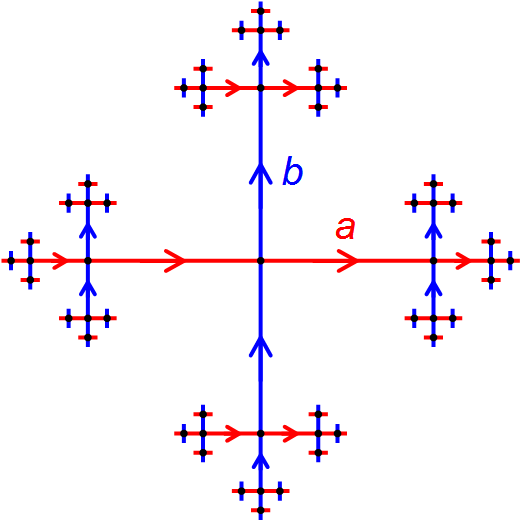
\includegraphics[height=2in]{cayley.png}
\caption{The Cayley graph of the free group over two elements, $a$ and $b$.}
\end{figure}

\subsection{Random Walk}

According to the level-crossing phenomenon, a random walk in one dimension will visit every node an infinite number of times.  We can test this phenomenon by performing a random walk on a one-dimensional graph.

\begin{verbatim}
(define-memoized (line x)
                 (make-vertex
                   (edges (line x)
                          ((line (1+ x)))
                          ((line (-1+ x))))
                   x))

(define (traverse-random vertex #!optional k)
  (let ((k (if (default-object? k) 1 k))
        (edges-stream (vertex-edges-stream vertex)))
    (if (or (eq? 0 k)
            (null? edges-stream))
      vertex
      (traverse-random
        (edge-head (stream-ref edges-stream
                               (random (stream-length edges-stream))))
        (-1+ k)))))
\end{verbatim}

\noindent By traversing randomly from \verb|(line 0)| and waiting to reach \verb|(line n)| for some $n$, we can count the number of steps it takes and verify that $n$ is indeed reached in finite time.

\subsection{Cover Time}

The cover time of a graph is the number of steps it takes in expectation to reach every vertex under a random walk.  We can take samples of the cover time by performing random walks on graphs.

\begin{verbatim}
(define (cover-time vertex)
  (let ((n (count-graph-vertices vertex))
        (done (make-eq-hash-table)))
    (let iter ((vertex vertex)
               (count 0))
      (hash-table/put! done vertex #t)
      (if (eq? n (hash-table/count done))
        count
        (iter (traverse-random vertex) (1+ count))))))
\end{verbatim}

\noindent Here, \verb|count-graph-vertices| counts the number of vertices in a graph.  We can compare the time it takes to cover a complete graph, a line graph, and a lollipop graph (a line graph attached to a complete graph at one end).

\begin{verbatim}
(define (make-lollipop n)
  (let ((clique (make-complete n))
        (line (make-line n)))
    (add-edge! (make-edge clique line))
    (add-edge! (make-edge line clique))
    clique))

(cover-time (make-complete 25)) ; 65
(cover-time (make-line 25))     ; 310
(cover-time (make-lollipop 25)) ; 13861
\end{verbatim}

\noindent The results match with the known asymptotic cover times of these graphs.

\subsection{Random Graphs}

Our graph library supports the construction of random graphs.  The edges present in a graph can be chosen randomly or edge weights and capacities can be chosen randomly.  We provide a simple example of a graph of $n$ vertices with edges chosen at random according to a Bernoulli distribution.

\begin{verbatim}
(define (make-numbered n filter #!optional properties)
  (let ((properties (if (default-object? properties)
                      (lambda (k x) '())
                      properties)))
    (define-memoized (vertex k)
                     (make-vertex
                       (make-edges
                         (stream-map
                           (lambda (head) (apply make-edge
                                                 (cons* (vertex k)
                                                        (vertex head)
                                                        (properties k head))))
                           (stream-filter (lambda (x) (and (filter k x)
                                                           (not (eqv? k x))))
                                          (stream-iota n))))
                       k
                       `(numbered ,n)))
    vertex))

(define (bernoulli p)
  (lambda (k x) (> 1 (random (exact->inexact (/ p))))))

(define (make-di-erdos n p)
  (make-numbered n (bernoulli p)))
\end{verbatim}

\noindent This example demonstrates the importance of memoization.  Because the vertices of the random graph are returned from a memoized function, their edges are generated only the first time they are referenced.  The second time a vertex is referenced, its edges are retrieved from its entry in the hash table, and the randomness provided to the memoized function is not used again.
\section{Conclusion}

The desire to succinctly represent common classes of graphs, in particular infinite graphs, motivated the design of a directed graph library based on lazy evaluation of edges. We can define graphs recursively in terms of adjacent vertices in a way that permits consistency across cycles by using memoized functions. Our system allows us to easily express graphs with a lot of symmetry.  In addition to providing a clear language for expressing graphs, our system supports running algorithms on graphs, including some algorithms on infinite graphs.

\subsection{Acknowledgments}

Thanks to Professor Gerald Sussman and Eli Davis for giving us guidance, providing us with past work, and teaching us how to build powerful programs.

\end{document}
